% Fig. 2 -- locality per task and under different conditions (figure*, Section 4)
\begin{figure*}[tbp]
  \centering
  \subcaptionbox{Per task: session share against cross-attempt share\label{fig:pertask}}{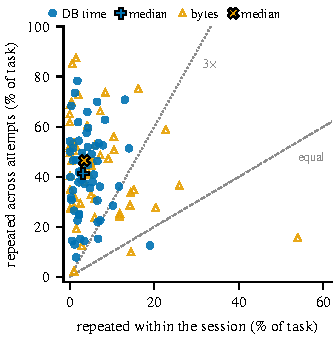
\includegraphics[height=2.05in]{figures/fig2a_pertask}}\hfill
  \subcaptionbox{Pooled share of isolated DB-execution time under different conditions\label{fig:conditions}}{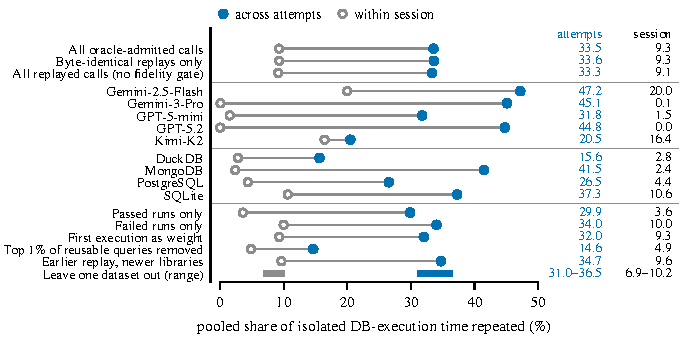
\includegraphics[height=2.05in]{figures/fig2b_conditions}}
  \caption{Locality per task and under different conditions. (a) One point per task and weight for the 54 tasks, on the oracle-admitted calls. Circles show isolated
  DB-execution time and triangles payload bytes. The axes give the share repeated within the session ($x$) and
  across attempts of the same task and model ($y$). The dashed line is $y=x$, the dotted line is
  $y=3x$, and large markers are task medians. (b) Pooled DB-time shares on the 70,173 oracle-admitted calls, a named
  subset, or another population. Byte-identical replays cover 66,556 calls, all replayed calls 76,141, and the earlier
  replay its 62,419 byte-identical calls. Shares are means over 200 random attempt orders, with 20 orders for the two
  gate variants and 50 for the top-1\% removal.}
  \label{fig:locality}
  \Description{Two panels. Left: a scatter plot with two points per task, one for DB time and one for bytes. Nearly all lie above the equal-share line and most above the three-times line. Right: one row per condition. The cross-attempt estimate lies to the right of the within-session estimate in every row, with the leave-one-dataset-out row shown as ranges.}
\end{figure*}
